\section{Clock Distribution}


% The resilience of the Clock Distribution translates into continuous and stable 
% synchronization of all the nodes and switches in the WRN (Table~\ref{tab:requirements}).
% A loss of time notion in a node can be caused by a link or switch failure - break of clock path 
% between the TM and the node. In order to prevent synchronization break, redundancy of network 
% elements (switches, cables) can be introduced ensuring redundant clock paths. However, 
% the switch-over between redundant elements might introduce instability and render the network 
% unreliable despite the costly redundancy. Therefore, the seamless switch-over between redundant 
% clock paths is one of the design-goals to enable network topology redundancy and, as a consequence, 
% offer robust and stable synchronization. The other reasons for the deterioration of synchronization 
% accuracy are the variation of external conditions (e.g. temperature) and loss of Ethernet frames with 
% timing information (PTP).  

%\subsection{Switch-over}

A seamless switch-over between redundant sources of timing (uplink ports) is heavily supported by 
the Clock Recovery System (CRS) \cite{biblio:TomekMSc} of the switch and the WR extension to PTP 
(WRPTP)\cite{biblio:WRPTP}. 

Figure~\ref{fig:switch-over} presents an example where a switch (timing slave) is connected 
(by its uplinks 1 \& 2) 
to two other switches (primary and secondary masters) -- the sources of timing. On both 
uplinks the frequency is recovered from the signal and provided to the CRS. Similarly, WRPTP 
measures delay and offset on each of the links and provides this data to the CRS. 
The modified Best Master Clock (mBMC) algorithm \cite{biblio:WRPTP} decides which of the 
timing masters is "better" and elects it the primary, the other is considered secondary (backup).
The information from {\it uplink 1} (primary) is used to control 
the CRS and adjust the local time. However, at any time all the necessary information from the 
{\it uplink 2} is available and a seamless switch-over can be performed in case of 
primary master failure \cite{biblio:TomekMSc}.

\begin{figure}[t]
\centering
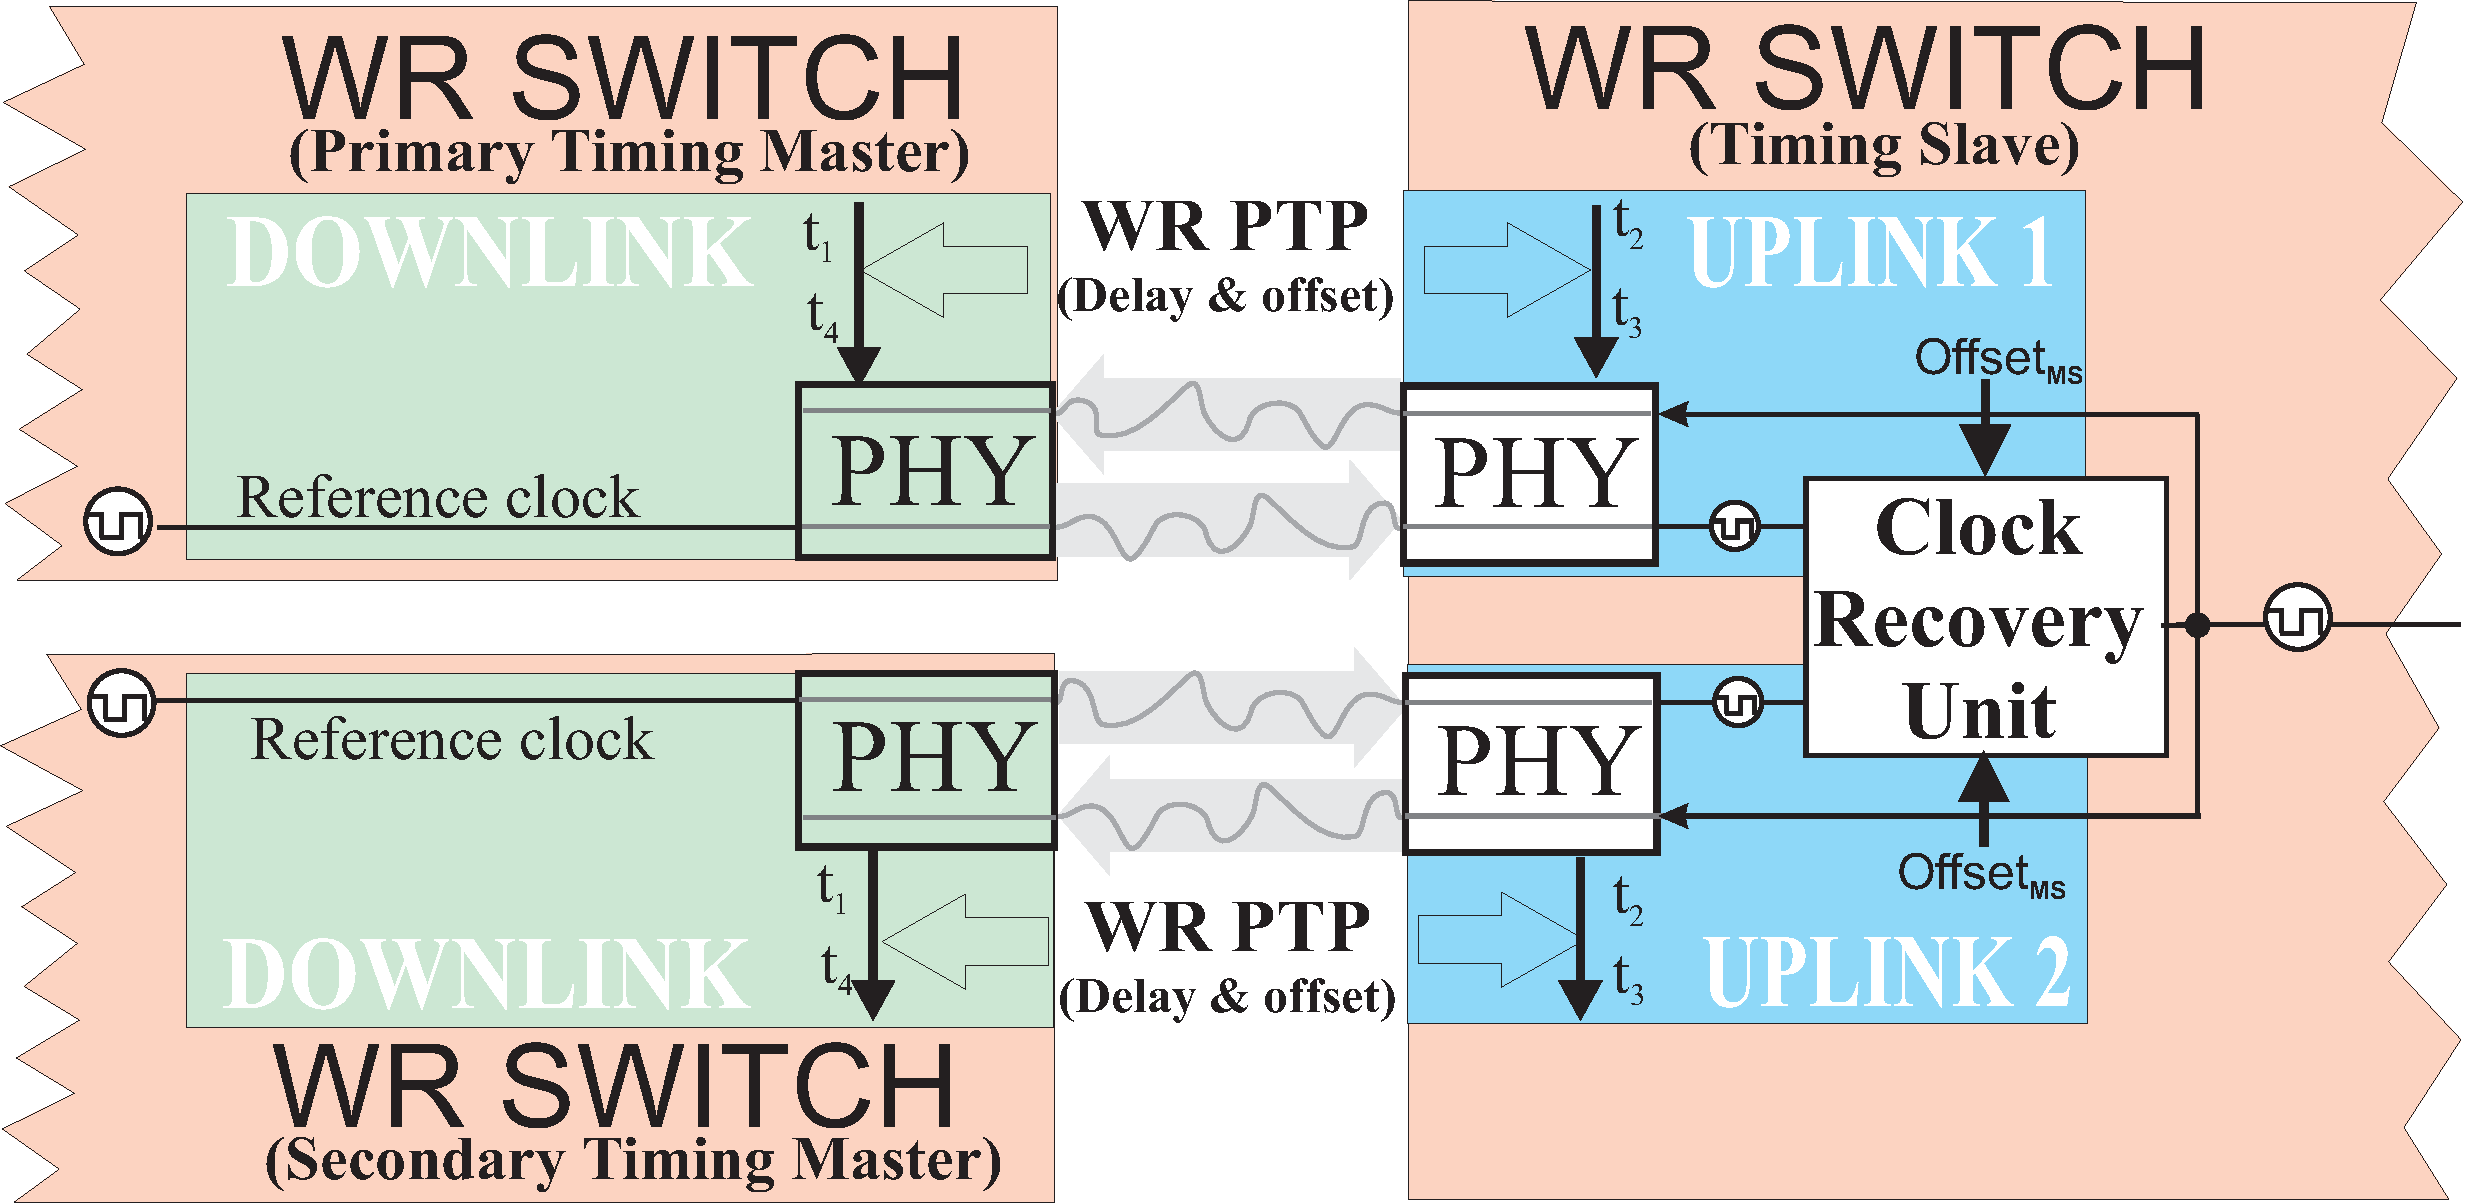
\includegraphics[width=3.2in]{robustness/clockDistribution.pdf}
\caption{Seamless switch-over.}
\label{fig:switch-over}
\end{figure}

%\subsection{Variable conditions and loss of PTP messages}
In addition to the switch-over-related synchronization instability, the variation of external temperature 
can cause an accuracy degradation. This problem, however, is solved by the PTP standard itself. By 
frequent link delay measurements, the fluctuation is compensated. 

